%------------------------------début entêtes-----------------------------------------
\pagestyle{fancy}

\renewcommand{\footrulewidth}{1pt}

\fancyhead[L]{\footnotesize \rightmark}
\fancyhead[C]{\thepage}
\fancyhead[R]{Contribution}

\fancyfoot[L]{Ny Hoavy Nomena}
\fancyfoot[C]{\thepage}
\fancyfoot[R]{Annotation automatique d'images}

%------------------------------fin entêtes-------------------------------------------

\chapter{Contribution au modèle théorique } \label{contribution}
\qquad Afin d'améliorer le modèle de génération de descriptions d'images proposé par Mao et al. dans \cite{mao2014deep} et \cite{mao2015learning} et présenté dans ce rapport en section \ref{presentationcontrib}, nous avons introduit dans ce dernier plus d'informations sur l'image. Ces informations sont représentées par un vecteur, nommé "vecteur de catégories". Ce vecteur représente les catégories (prédéfinies dans la collection de données) détectées et non détectées sous forme de scores. \\
\smallskip


\section{Présentation de la contribution} \label{presentationcontrib}
\qquad Inspirée de \cite{jia2015guiding} \cite{xu2015show}, notre bjectif est d'intégrer plus d'informations sémantiques, dans les modèles de génération de descriptions pour les améliorer. \cite{jia2015guiding} propose une extension du LSTM nommée gLSTM (pour guided LSTM). A la différence du LSTM, gLSTM prend  des informations sémantiques issues de l'image comme entrées supplémentaires. Dans les modèles LSTM \cite{mao2014deep} \cite{vinyals2015show} \cite{donahue2015long}; \cite{jia2015guiding} a affirmé que  les phrases générées dévient du (ne correspondent pas au) contenu de l'image à cause du comportement instable du décodeur : d'une part la phrase générée doit décrire le contenu de l'image  et d'une autre elle doit être un modèle de langue qui définit la séquence de mots la plus envisageable (suivant le contexte et les règles grammaticales). Pour insister sur le contenu de l'image, \cite{xu2015show} a introduit un mécanisme d'attention visuelle.
Dans \cite{xu2015show}, le mécanisme d'attention est représenté par un contexte qui se réfère à une information visuelle capturée sur des régions de l'image. Ainsi les unités du décodeur accordent plus d'attention sur des régions particulières de l'image pour générer la séquence de mots.
Le contexte est un vecteur calculé à partir de deux types de mécanisme d'attention : stochastique et déterministe \footnote{l'explication n'est pas à la portée de ce rapport voir \cite{xu2015show}}. \cite{jia2015guiding} ont utilisé des informations sémantiques de l'image pour guider le modèle de langue. Leur contribution est une extension du LSTM : gLSTM qui, par addition, prend en entrée l'information sémantique de l'image  pour orienter le décodeur à favoriser les mots qui sont liés au contenu de l'image. Concrètement, l'information sémantique est ajoutée en entrée dans les unités (\textit{gates}) du LSTM.\\
Le gLSTM redefinie les unités de LSTM par:\\
$\begin{matrix}
i_{t}=\sigma(W^{(i)}x_{t}+ U^{(i)}h_{t-1} + V^{(i)}g) & input\, gate\\ 
f_{t}=\sigma(W^{(f)}x_{t}+ U^{(f)}h_{t-1} + V^{(f)}g )& forget\, gate\\
o_{t}=\sigma(W^{(o)}x_{t}+ U^{(o)}h_{t-1} + V^{(o)}g)  & output\, gate\\ 
\check{c}_{t} = \tanh(W^{(c)}x_{t}+ U^{(c)}h_{t-1}) & new\, memory\, cell\\
c_{t}=f_{t} \circ c_{t-1}+i_{t} \circ \check{c}_{t} & final\, memory\, cell\\
h_{t}=o_{t} \circ \tanh(c_{t})& hiden state 
\end{matrix}$

$g$ est le vecteur représentatif de l'information sémantique.\\

Nous proposons une autre alternative pour une extension des modèles de base présentée dans les paragraphes suivants.

Dans notre travail, l'information sémantique d'une image est représentée par un vecteur de scores des catégories: vecteur de catégories. Le vecteur de catégories $V_{cat}$ [figure \ref{fig:vcat}] est composé de scores attribués à chaque catégorie pour une image. Cette information permet de guider le modèle à former des phrases plus adaptées au contenu de l'image. Cette hypothèse est justifiée par le fait que la description d'une image est surtout générée à partir des catégories auxquelles elle appartient (exemple [figure \ref{fig:vcat}]).\\

\medskip
\begin{figure}[h]
	\begin{center}
	\label{fig:vcat}
		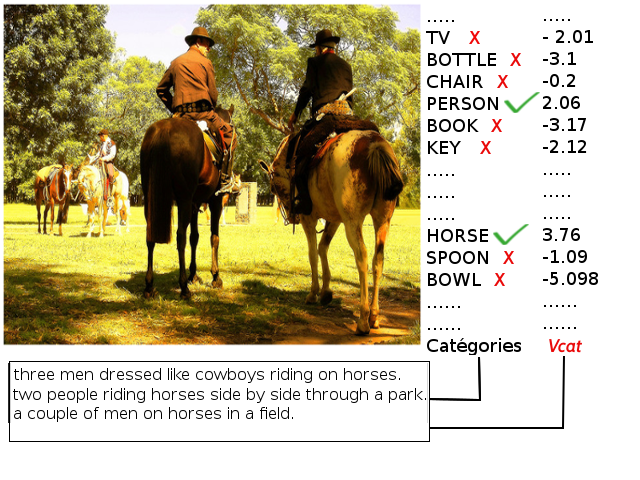
\includegraphics[width=0.4\textwidth]{vcat}
		\caption{Illustration de la relation entre catégories, $V_{cat}$ et descriptions}
	\end{center}
	Les descriptions se rapportent aux catégories auxquelles l'image appartient (person, horse). Notre modèle de classification est entraîné pour prédire ces catégories et leur assigne des scores positifs et pour les autres catégories des scores négatifs. Ces scores forment le vecteur $V_{cat}$. 
\end{figure}

Ainsi, on peut redéfinir l'estimation de la loi de probabilité de la séquence sachant la caractéristique visuelle de l'image $I$: $V(I)$ (issu du réseau de neurones convolutifs) et l'information  $V_{cat}(I)$ lors de la classification des images:
\begin{eqnarray}
\label{eq:lp}
P(w_{i}| W_{1:i-1}, V(I), V_{cat}(I))
\end{eqnarray}
L'equation \ref{eq:lp} représente la probabilité de générer un mot $w_{i}$.

Pour cela, les travaux que nous avons effectués comportent deux parties :
\begin{itemize}
	\item classification : détaillée dans la section \ref{classification}, est la partie dans laquelle les réseaux de neurones convolutifs sont utilisés pour classifier les images dans des catégories prédéfinies dans les données d'apprentissage. Le modèle est utilisé pour prédire les catégories auxquelles une image en entrée appartient. Ce modèle attribue à chaque catégorie un score qui va former le vecteur de catégories.
	\item génération de descriptions : détaillée dans la section \ref{gendesc}, utilise les résultats de la classification pour apporter l'information sur l'image. Le vecteur de catégories est utilisé comme entrée additionnelle dans notre modèle de base pour estimer la loi de probabilité (\ref{eq:lp}). Le modèle de base de notre contribution est un réseau de neurones récurrents multimodal de Juan Mao et al. dans \cite{mao2014explain} \cite{mao2014deep} et \cite{mao2015learning}
\end{itemize}

\subsection{Classification des images} \label{classification}

\qquad Les méthodes de classification ne prennent pas en compte la signification des textes associés aux images. Leur objectif est de classer les images selon les catégories prédéfinies considérées.\\
Dans les travaux cités sur la reconnaissance de formes et d'objets \ref{vo}, les modèles sont entraînés pour prédire une seule catégorie pour une image donnée. Dans notre cas, une image peut appartenir à plusieurs catégories à la fois. Par exemple, l'image d'un chien et de son maître appartient à la catégorie chien et personne à la fois. La classification multi-labels est alors utilisée pour permettre une association multiple entre une image et les catégories.
	Pour une classification multi-labels, le modèle est entraîné pour prédire les catégories auxquelles une image appartient par estimation de la fonction :
$f : X \rightarrow 2^Y $ pour une donnée d'apprentissage : ${(x_1, Y_1), (x_2,Y_2),…, (x_m,Y_m)}$.
$x_i \in X$ est une instance de l’i-ème image en entrée représentée par le vecteur descripteur.
$Y_i = {y_{i1},..,y_{il_{i}}} \subset Y$ est l'ensemble des labels ou catégories associés à l'i-ème image . $l_i$ est le nombre de catégories associées à cette image.
\medskip
\begin{figure}[h]
	\begin{center}
		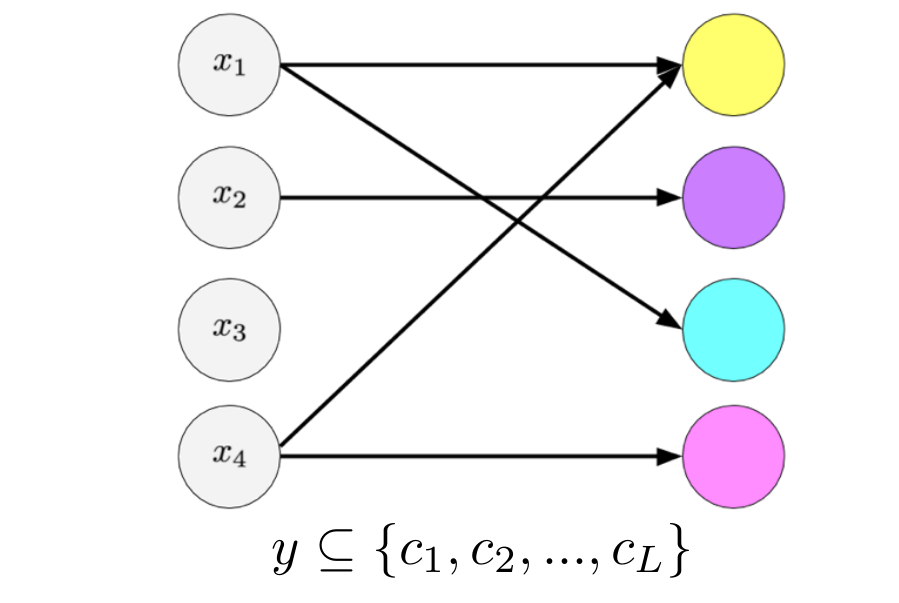
\includegraphics[width=0.3\textwidth]{multilabel}
		\caption{Classification multi-labels}
	\end{center}
\end{figure}

Notre objectif est d'extraire le vecteur de catégories composé de score de chaque catégorie pour une image donnée. Notre modèle a été entraîné pour assigner des scores positifs pour les catégories auxquelles l'image appartient et négatifs aux autres. L'apprentissage a été effectué par réglage fin d'un réseau de neurones convolutifs pré-entrainé en optimisant la fonction objectif entropie croisée (equation \ref{entropie}).\\
\begin{eqnarray}
\label{entropie}
E = \frac{-1}{n} \sum_{n=1}^{N} [p_n \log \hat{p}_n + (1-p_n) \log(1- \hat{p}_n)].
\end{eqnarray}
$\hat{p}_n = \sigma(x_n) \in [0,1]$\\
$\sigma$ est la fonction sigmoïde \\
$x_n$ est le score prédit par le modèle pour la catégorie $n$\\
$p_n = 1$ si l'image appartient à la catégorie $n$ et $0$ sinon\\ 

Le vecteur de catégories est extrait par propagation directe de l'image sur notre modèle. On définit  pour une image $I$ : $V_{cat}(I) = f_{multilabel}(I)$.\\
$V_{cat}(I) \in \mathbb{R}^{C}$. $C$ est le nombre de catégories prédéfinies de la collection de données.

\subsection{Génération de descriptions utilisant le vecteur de catégories} \label{gendesc}

\qquad Notre contribution a été intégrée dans le modèle de base \cite{mao2014explain} \cite{mao2014deep} nommé m-RNN pour\textit{ multimodal Reccurent Neural Network} en anglais. L'architecture de ce modèle nous permet d'expérimenter l'efficacité de l'utilisation du vecteur de catégories pendant l'apprentissage d'un modèle de génération de descriptions.

\medskip
\begin{figure}[h]
	\begin{center}
		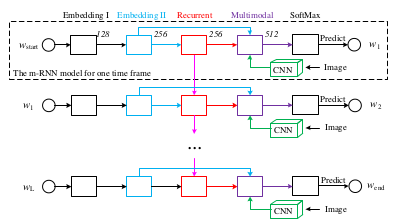
\includegraphics[width=0.6\textwidth]{mrnn}
		\caption{modèle de base m-RNN  \cite{mao2014deep}}
	\end{center}
\end{figure}

Le modèle m-RNN est composé :
\begin{itemize}
	\item d'un modèle de langue pour la représentation des mots et  phrases
	\item d'un composant visuel pour la représentation des images
	\item d'un composant multimodal pour combiner les différentes représentations des informations
\end{itemize}

Dans le modèle de langue, chaque phrase est représentée par un sac-de-mots binaire selon l'index du mot dans le vocabulaire. Deux couches de neurones successives sont utilisées pour la représentation vectorielle des mots par la méthode de \textit{word embedding}. Cette représentation est ensuite propagée dans un réseau de neurones récurrents et dans le composant multimodal. Le réseau de neurones récurrent (LSTM ou GRU) est utilisé pour stocker le contexte dans l'état caché.\\
\qquad	Le composant visuel est un vecteur caractéristique $I$ de l'image issue d'un réseau de neurones convolutifs pré-entrainé (15-ème couche de VGG-16).
	Le composant multimodal relie ces 3 sorties : du word embedding, du RNN et du composant  visuel pour prédire les mots de la séquence  sachant l'image.
	
Pour une formulation mathématique, nous allons adopter la notation suivante :\\
à un instant $t$, soient\\
$w(t)$ : la représentation finale du mot issu de la seconde couche de word embedding,\\
$h(t)$ : l'activation (sortie) du RNN,\\
$f_2(x)$ : la fonction ReLu,\\
$I$ : le vecteur caractéristique de l'image issu du réseau de neurones convolutifs,\\
$m(t)$ : l'activation de la couche multimodale.\\

\begin{eqnarray}
r(t) = f_2(U_r r(t-1)+w(t))
\end{eqnarray}\\
\begin{equation}
\label{equ:multimodalorig}
m(t) = g_2(V_w w(t)+V_r r(t)+ V_I I)
\end{equation}
$U_r$ est une matrice de projection de l'activation du RNN à l'instant $t-1$ sur le même espace
% de vecteur (espace vectoriel) 
que $w(t)$.\\
L'activation de la couche multimodale est obtenue par la somme des projections des 3 sorties dans un même espace : l'espace multimodal.\\
La sortie du modèle est une couche $softmax$ qui produit la probabilité de générer chaque mot du vocabulaire à partir de la couche multimodale.
% en utilisant la stratégie du \textit{« Transposed Weight Sharing»} partage de poids transposé \cite{mao2015learning}.\\

Le modèle est entraîné par rétropropagation en optimisant la fonction logarithme de la vraisemblance. La fonction objectif du modèle calcule la moyenne de la fonction  de vraisemblance logarithmique sur les mots sachant le contexte et l'image correspondant dans les phrases d'apprentissage.\\
\begin{eqnarray}
C = \frac{1}{N} \sum_{i=1}^{N_{S}} L_{i} \log_{2} PPL(w_{1:L_{i}^{(i)}}| I^{(i)}) + \lambda_{\theta} ||\theta||^{2}_{2}
\end{eqnarray}\\
$N_{S}$: nombre de phrases de références\\
$N$ : nombre de mots\\
$L_i$ : longueur de l'i-ème phrase\\
$PPL(w_{1:L_{i}}| I)$ :  est la perplexité (mesure standard pour les modèles de langue) de la phrase $w_{1:L}$ sachant l'image $I$:
\begin{eqnarray}
\log_{2} PPL(w_{1:L_{i}}| I) = - \frac{1}{L} \sum_{n=1}^{L} \log_{2} P(w_n|w_{1:n-1},I)
\end{eqnarray} 
$P(w_n|w_{1:n-1},I)$ est obtenu sur l'activation de la couche $softmax$ et représente la probabilité à générer  le mot $w_n$, sachant $I$ et les mots précédents $w_{1:n-1}$.

Dans notre modèle, on a introduit un autre composant qui apporte au modèle d'origine plus d'information sémantique sur le contenu de l'image. Ce composant projette le vecteur de catégories associé à l'image $I$: $V_{cat}(I)$ dans l'espace multimodal  afin de générer le futur mot  de la séquence. Ainsi l'équation \ref{equ:multimodalorig} devient: 
\begin{equation}
\label{equ:multimodalcontr}
m(t) = g_2(V_w w(t)+V_r r(t)+ V_I I + V_c V_{cat}(I))
\end{equation}

\section{Implémentations} \label{implementation}

Pour la partie classification, nous avons utilisé l'environnement  "caffe"\cite{jia2014caffe}. La classification multi-labels est effectuée par réglage fin (ajustement) du modèle pré-entrainé VGG-16 d'Oxford \cite{simonyan2014very}. La couche softmax a été remplacée par une fonction sigmoïde entropie croisée pour l'apprentissage.\\
%detail de l'apprentissage
Le modèle a été entraîné par descente de gradient stochastique sur des lots de taille 128 et avec un taux d'apprentissage de 0.0001.

Pour la génération de descriptions, notre implémentation s'est basée sur une implémentation sur tensorflow \cite{abadi2016tensorflow} du modèle m-RNN disponible pour tout public \footnote{github.com/mjhucla/TF-mRNN}. Un modèle préentrainé de l'inception V3 a été utilisé comme descripteur pour extraire les vecteurs caractéristiques visuels des images. \\
Les phrases associées ont été prétraitées comme suit:  elles ont été segmentées en séquence de mots. Les mots qui apparaissent moins de cinq fois dans le corpus entier sont filtrés et ne sont pas inclus dans le vocabulaire et sont remplacés par le caractère  $<unk>$.

Notre expérimentation concerne 4 modèles. 
\begin{itemize}
	\item Le premier modèle est le modèle de base de notre contribution \cite{mao2014deep} \cite{mao2015learning} désigné par "modèle de base".
	\item Le second modèle "modele-init" est un modèle inspiré par show and tell  \cite{vinyals2015show} et deep visual aligment \cite{karpathy2015deep} qui consiste à initialiser l'état caché du modèle de langue par le vecteur caractéristique visuel.
	\item Le troisième modèle est un modèle utilisant des vecteurs de catégories tirés directement à partir des données d'apprentissage. Ce modèle correspond à une version optimale du modèle de notre contribution. Il représente le modèle de notre contribution quand toutes les catégories auxquelles une image appartient sont prédites à $100\%$.
%Il est équivalent au modèle de notre contribution qui peut prédire à $100\%$  exactement tous les catégories auxquelles une image appartient.
	\item Le quatrième modèle est notre modèle qui utilise des vecteurs de catégories prédits par le modèle de classification précédente.
\end{itemize}
Ces modèles utilisent une même configuration donnée par le tableau \ref{table:config}.

% batch_size = 64
% mumtimodal size:2048
% embedding_size = 1024
%learning rate 1.0 
%nombre de couches	: 1
\begin{table}
\caption{Configuration utilisée par les quatre modèles}
\label{table:config}
\fontsize{8}{12}\selectfont
\begin{tabular}{|c|M{3cm}|M{3cm}|c|c|}
    \hline
     taux d'apprentissage & dimension du composant multimodal & dimension de l'encapsulation  & nombre de couche RNN& Beam size\footnotemark  \\
	\hline
    1.0 & 2048 & 1024 & 1 &3\\ 
    \hline  
\end{tabular}
\end{table}
\footnotetext{Beam search: Considérer itérativement les $k$ meilleures séquences à l'intant $t$ pour générer les séquences en $t+1$. $k$ est appelé \textit{beam size}} 
\chapter{Évaluation de notre proposition}
\section{Ressources expérimentales} \label{ressources}

Les ressources utilisées lors de notre expérimentation sont similaires à celles utilisées dans le modèle de base \cite{mao2014deep} \cite{mao2015learning} pour une meilleure comparaison des résultats et l'estimation de l'amélioration effectuée sur ce modèle.

\subsection{Collection de données :}
%Amazon Mechanical Turk Amazon Mechanical Turk is crowdsourced Internet marketplace for tasks that computers are currently unable to do. (https://www.mturk.com)

La collection de données utilisée est la collection de Microsoft Common Objects in COntext : MS COCO cite{lin2014microsoft}. MS COCO  est une des collections les plus utilisées pour l'expérimentation des modèles de génération de descriptions comme Flickr8k \cite{hodosh2013framing} Flickr30k \cite{young2014image}. MS COCO contient des images naturelles classées dans 90 
%« choses »[sont des catégories incluants les objets qui sont facilement localisés comme personne, chaise, voiture] et « truc » [sont des catégories difficiles à segmenter comme ciel, herbe, route]
catégories. La majorité des images de cette collection sont des images non iconiques  qui permettent aux modèles de mieux généraliser lors de leur apprentissage.\\
Nous avons utilisé la collection MS COCO Captions \cite{chen2015microsoft} qui utilisent les images collectées par MS COCO issus de 80 catégories d'objets et de scènes. Dans sa version actuelle, MS COCO Caption contient 82,783 images d'apprentissage et 40,504 images de validation. Chaque image est annotée par cinq phrases descriptives.

Avec cette collection de données, nous avons généré 13691 mots dans le vocabulaire. Pour l'apprentissage des modèles, nous avons utilisé les 80.000 images d'apprentissage de la collection. Pour évaluer les modèles, nous avons extrait aléatoirement sur les images de validation: 4000 images pour la validation et 1000 images pour le test. 
\\
\medskip
\begin{figure}[h]
	\begin{center}
		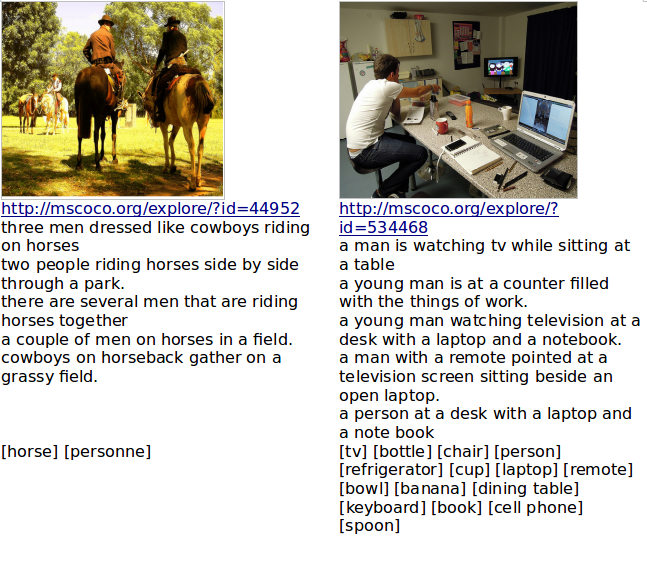
\includegraphics[width=0.7\textwidth]{mscococaptioning}
		\caption{Exemples de données dans Microsoft COCO Captions \cite{chen2015microsoft}}
	\end{center}
\end{figure}


\subsection{Mesures d'évaluation}

\subsubsection{Mesures d'évaluation de la classification :}
\qquad Pour la classification multi-labels, notre modèle est évalué par quatre mesures.\\
Soient $Y_i$ l'ensemble des labels corrects pour une instance donnée $i$ et $\hat{Y}_i$ l'ensemble des labels prédits par notre modèle pour cette instance.

L'erreur de Hamming (hamming loss en anglais) mesure, en moyenne, l'erreur commise par le modèle sur la prédiction de chaque label. Elle prend en compte les labels prédits incorrects et les labels pertinents non-prédits.
\begin{eqnarray}
hamming loss = \frac{1}{NL} \sum_{i=1}^{N} \sum_{j=1}^{L} [I(j \in \hat{Y}_{i} \wedge j \notin Y_{i} ) + I(j \notin \hat{Y}_{i} \wedge j \in Y_{i} )].
\end{eqnarray}

La distance de Hamming est aussi utilisée pour compenser l'erreur de Hamming lors de la mesure de la performance du modèle. Elle est donnée par l'équation \ref{eq:hammingdist}.
\begin{eqnarray}
hamming distance = \frac{1}{NL} \sum_{i=1}^{N} \sum_{j=1}^{L} [I(j \in {Y}_{i} \wedge j \in \hat{Y_{i}} )].
\label{eq:hammingdist}
\end{eqnarray}

L'accuracy pour chaque instance est définie comme la proportion des labels corrects prédits sur le nombre total de labels de cette instance. L'accuracy est la moyenne sur toutes les instances considérées.
%L'accuracy: Accuracy for each instance is defined as the proportion of the predicted correct labels to the total number (predicted and actual) of labels for that instance. Overall accuracy is the average across all instances
\begin{eqnarray}
Accuracy = \frac{1}{N} \sum_{i=1}^N \frac{\|Y_i \cap \hat{Y}_i\|}{\|Y_i \cup \hat{Y}_i\|}
\end{eqnarray}

La mesure "exact match ratio" est une mesure qui ne prend pas en compte les prédictions partiellement correctes mais les considère comme incorrectes. Elle est définie par l' equation \ref{eq:mr}.
\begin{eqnarray}
MR = \frac{1}{N} \sum_{i=1}^{N}I(Y_i = \hat{Y}_i)
\label{eq:mr}
\end{eqnarray}
$I$ est la fonction indicatrice.
$N$ est le nombre d'instances considérées.

\subsubsection{Mesures d'évaluation des descriptions générées:}

Une description est jugée selon sa signification (elle doit décrire avec précision l'image) et sa syntaxe (elle doit être grammaticalement correcte). Cependant, aucune mesure n'est aujourd'hui appropriée pour l'évaluation automatique de ces critères \cite{young2014image} \cite{ordonez2011im2text}. L'évaluation automatique des descriptions générées s'inspire donc des mesures utilisées pour évaluer les systèmes de traduction et de génération de résumés. Dans notre cas, les mesures sont les mêmes utilisées dans le concours MS COCO Captions \cite{chen2015microsoft}.
%BLEU \cite{papineni2002bleu}, ROUGE \cite{lin2004rouge}, METEOR \cite{denkowski2014meteor} et CIDEr \cite{vedantam2015cider} qui a été élaboré particulièrement pour l'évaluation des descriptions des images.\\
\smallskip

L'évaluation s'applique sur la qualité des descriptions générées (phrases candidates) par rapport aux descriptions dans la collection (phrases de références) sachant une image donnée.
Pour la suite, nous avons adopté la notation citée dans \cite{chen2015microsoft} pour la définition des mesures d'évaluation des modèles entraînés sur cette collection \cite{mao2014deep} \cite{mao2015learning} \cite{fang2015captions} \cite{xu2015show} \cite{karpathy2015deep} \cite{donahue2015long}. L'évaluation automatique mesure pour une image $I_{i}$ la description candidate $c_{i}$ sachant un ensemble de descriptions de références $S_{i} = \left \{ s_{i1},..., s_{im} \right \}$ appartenant à $S$.
Les phrases descriptives sont représentées par un ensemble de n-grammes.
$h_{k}(s_{ij})$ est le nombre d'occurrence d'un n-gramme $w_{k}$ dans une phrase $s_{ij}$.
$h_{k}(c_{i})$   est le nombre d'occurrence d'un n-gramme $w_{k}$ dans les candidats $c_{i}$ appartenant à $C$

\paragraph{BLEU \cite{papineni2002bleu}:} 
BLEU est utilisée pour l'évaluation des systèmes de traduction. Ce type de mesure analyse la cooccurrence des n-grammes entre les phrases générées $C$ et les phrases du corpus de référence $S$.
Soit la précision entre les phrases coupées en n-gram $CP_{n}(C,S)$
\begin{equation}
CP_{n}(C,S)=\frac{\sum_{i}\sum_{k} \min(h_{k}(c_{i}),\underset{j\in m}{\max}h_{k}(s_{ij}))}{\sum_{i}\sum_{k} h_{k}(c_{i})}
\end{equation}
$k$ : index de l'ensemble des n-gram possibles

Cette précision $CP_{n}(C,S$) est accompagnée d'une \textit{pénalité de brièveté} de la phrase $b(C,S)$ du fait qu'elle favorise les phrases courtes \cite{papineni2002bleu}.\\
%destinée à pénaliser les systèmes qui essaieraient d’augmenter artificiellement leurs scores en produisant des phrases délibérément courtes.
$
b(C,S)=\left\{\begin{matrix}
1 & si \, l_{C}>l_{S}\\ 
e^{1-l_{S}/l_{C}} & si \, l_{C}\leq l_{S}
\end{matrix}\right.
$
\\
$l_{C}$ et $l_{S}$ sont les longueurs totales respectives des phrases candidates $c_i$ et du corpus de référence.

La mesure BLEU est calculée par :
\begin{eqnarray}
BLEU{N}(C,S)=b(C,S) \exp \left (  \sum_{n=1}^{N} w_{n} \log CP_{n}(C,S)  \right )
\end{eqnarray}
%wn sont des poids positifs tq leur sommes =1 s
$N = 1, 2, 3, 4$ (BLEU-1, BLEU-2, BLEU-3, BLEU-4)
\\
\qquad	Selon \cite{chen2015microsoft}, BLEU a montré de bonnes performances pour les comparaisons au niveau du corpus sur lequel un grand nombre de  n-gram sont identiques. Cependant pour une comparaison (individuelle) entre les n-grammes des phrases, les correspondances ne se produisent que rarement. Ainsi BLEU n'est pas très appropriée pour la comparaison phrase à phrase.
	Cette mesure est utilisée dans la génération de description pour comparer les descriptions générées (phrases candidates) par le modèle et les descriptions issues de la collection de données (corpus de référence).
%desavantage: mesure de performance qui peut depasser celle des humains

%\paragraph{ROUGE \cite{lin2004rouge}:} 
%
%\qquad	Notre modèle de base \cite{mao2014deep} \cite{mao2015learning} ont été évalués par la mesure $ROUGE_L$ qui est basée sur le plus long sous-séquence commun « Longest Common Subsequence  LCS». $ROUGE_L$ est obtenue par calcul d'une F-mesure :
%\begin{eqnarray}
%R_{l}= \underset{j}{max} \frac{l(c_{i}, s_{ij})}{|s_{ij}|}\\
%P_{l}= \underset{j}{max} \frac{l(c_{i}, s_{ij})}{|c_{i}|}\\
%ROUGE_{L}(c_{i},S_{i})=\frac{(1+\beta^{2})R_{l}P_{l}}{R_{l}+\beta^{2}P_{l}}
%\end{eqnarray}
%
%$ l(c_{i}, s_{ij})$ : est la longueur du LCS entre la phrase candidate ci et la phrase référence sij
%$ R_{l}$ est le rappel et $P_{l}$ est la précision du LCS
%$\beta = 1.2 $

\paragraph{METEOR \cite{denkowski2014meteor}:} 
%Un alignement est effectué entre une hypothèse de reconnaissance et la phrase de référence. 
Un alignement est effectué entre les mots de la phrase candidate et de la phrase de référence.
%L'alignement est calculé tant que le nombre de morceaux $ch$ (chunk) de token \footnote{voir tokenisation} contigües et identiquement ordonnées  des deux phrases est minimisé.\\
L'alignement est calculé en réduisant le nombre de morceaux  $ch$ (chunk)  contiguës et identiquement ordonnées  des deux phrases.
Soit $m$ un ensemble d'alignements, METEOR est une moyenne harmonique de la precision $P_m$ et le rappel $R_m$ entre les phrases de référence et les phrases candidates. Le score final inclut une pénalisation $Pen$ calculée sur le nombre de mots qui se correspondent $m$ et le nombre de morceaux $ch$ pour prendre en compte l'ordre des mots des séquences générées.
donné par :
\begin{eqnarray}
Pen= \gamma \left ( \frac{ch}{m} \right )^{\theta}\\
R_{m}= \frac{|m|}{\sum_{k}h_{k}(s_{ij})}\\
P_{m}= \frac{|m|}{\sum_{k}h_{k}(c_{i})}\\
F_{mean} = \frac{P_{m}R{m}}{\alpha P_{m}+(1-\alpha)R_{m}}\\
METEOR=(1-Pen)F_{mean}
\end{eqnarray}

%Un alignement peut être défini comme un ensemble de correspondances d’uni-grammes. Un uni-gramme d’une phrase est mis en correspondance avec zéro ou un seul uni-gramme d’une référence.
%Les correspondances sont basées en premier lieu sur des formes orthographiques identiques, puis sur des mots de même racine (stemmisation) et enfin sur les synonymes. Cet alignement permet de mieux évaluer les hypothèses en tenant compte de plusieurs possibilités lexicales différentes de la référence. Le meilleur alignement est celui qui contient le plus grand nombre de correspondance d’uni-grammes avec le plus petit nombre de réordonnancements. Le score METEOR est déterminé à partir de ce meilleur alignement. Le score METEOR (qui paraît assez efficace) dépend de la disponibilité des dictionnaires ce qui n’est pas évident dans toutes les langues.
%more intelligent, uses WordNet and doesn't penalize similar words
%paramètre par defaut: alpha = 0.85, beta = 	0.20, gamma = 0.60, delat = 0.75
\paragraph{CIDEr \cite{vedantam2015cider}}
Cette mesure est propre à l'évaluation des modèles de génération de légendes et est la mesure la plus corrélée avec le jugement humain \cite{vinyals2016show}.

CIDEr mesure un consensus dans les descriptions en calculant le TF-IDF (Term Frequency Inverse Document Frequency) pondéré pour chaque n-gramme. CIDEr calcule le TF-IDF pondéré pour chaque n-gramme par :
\begin{eqnarray}
g_{k}(s_{ij})= \frac{h_k(s_{ij})}{\sum_{\omega_{l}\in \Omega}h_{t}(s_{ij})} \log \left(\frac{|I|}{\sum_{I_{p}\in I}min \left ( 1,\sum_{q}h_{k}(s_{pq}) \right) } \right )
\end{eqnarray}

$\Omega$ est le vocabulaire pour les n-grams\\
$I$ est l'ensemble des images\\
Le premier terme mesure le TF pour chaque n-gram $w_{k}$ et le second terme calcule l'IDF.

Pour un n-gram, $CIDEr _{n}$ est obtenu par une moyenne de la distance entre la phrase candidate et les phrases références (estimé par le rappel et la précision)
\begin{eqnarray}
CIDEr_{n}(ci,S_{i})= \frac{1}{m} \sum_{j} \frac{g^{n}(c_{i}).g^{n}(s_{ij})}{\left \|g^{n}(c_{i})  \right \| \left \|g^{n}(s_{ij})  \right \|}
\end{eqnarray}\\
$g^n(u)$ est un vecteur formé par les $g^k(u)$ correspondant aux n-grams.\\
$\left \|g^{n}(u)  \right \| $ est la norme du vecteur $g^n(u)$.\\
$u : c_{i}$ ou $s_{ij}$.\\
En sommant sur les n-gram :
\begin{eqnarray}
CIDEr(c_{i},S_{i})=\sum_{n=1}^{N} w_{n}CIDEr(c_{i},S_{i})
\end{eqnarray}\\
$ w_{n} = 1/N $ avec $N=4$ dans notre cas.
\\
%Goal: measure “human-likeness” - does sentence sound like it was written by a human?
% CIDEr: Consensus-based Image Description Evaluation
%Use Mech Turk to get human consensus
%Do not provide an explicit concept of similarity; the goal is to get humans to dictate what similarity means
%Measure of consensus should encode how often n-grams in candidate sentence are present in references
%More frequent n-grams in references are less informative if n-gram is in candidate

Ces mesures d'évaluation ont été utilisées dans le concours organisé par MS COCO Captioning \footnote{http://mscoco.org/dataset/\#captions-challenge2015 http://mscoco.org/dataset/\#captions-eval}; nous les utilisons également dans notre évaluation.

